\chapter{Results}
\label{chap:results}
In order to visually demonstrate the encryption, visualisations of the ciphertext polynomial $c_0$ (refer to \cref{sec:ckks}) were generated using a \gls{crt} decomposition of the \gls{rns} representation of $c_0$.
Each pixel corresponds to a coefficient $a \in \Z / q\Z$ scaled down by the modulus $q$ to obtain a brightness value between $0$ and $1$.

\begin{figure}[H]
  \centering
  % 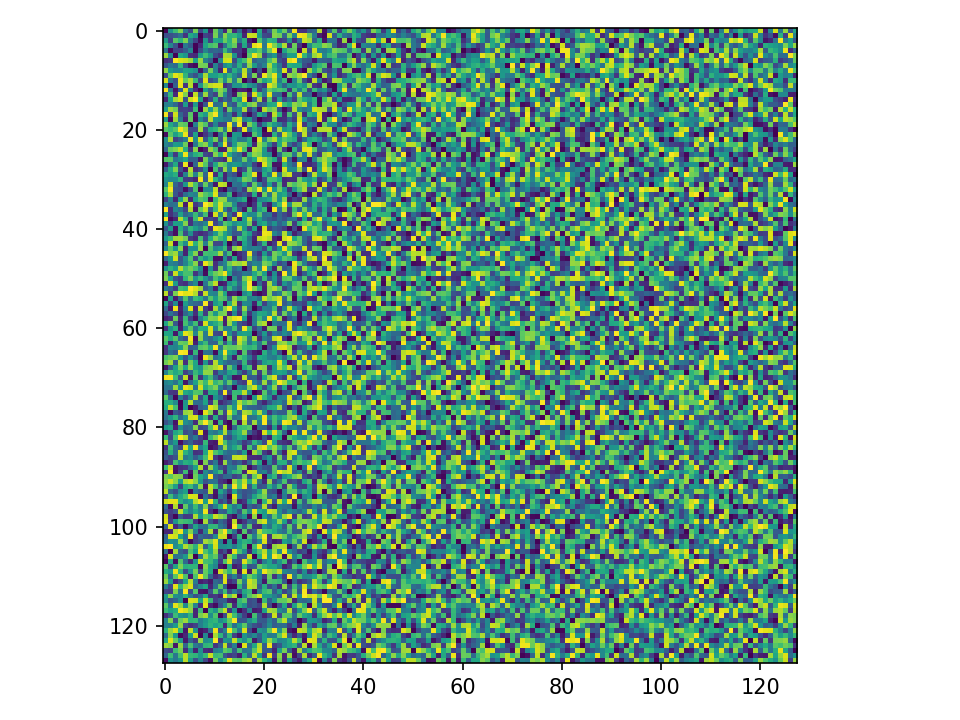
\includegraphics[width=\linewidth]{figures/ciphertext-visualisation.png}
  \inputtikz{figures/ciphertext-visualisation}
  \caption[Visualisation of the plain input images compared to their ciphertext]{Ciphertext Visualisation: The first row corresponds to the images in plain, the second row depicts an encrypted version, namely the reconstructed polynomial coefficients $a_k$ of the ciphertext polynomial.}
  \label{fig:ciphertext-visualisation}
\end{figure}

\begin{figure}[H]
  \centering
  \pgfplotsset{/pgfplots/group/.cd,vertical sep=1.6cm}
  \inputtikz{figures/generated/training-history}
  \caption[Classification accuracy and loss development during training]{Development of the classification accuracy and the mean squared error during training.}
  \label{fig:training-history}
\end{figure}

The machine learning framework behind the project, Tensorflow, splits its training process into \textit{epochs}, which can be found on the x-axis in the plot above.
For each training epoch, we find the progress that has been made in a single epoch by looking at the new accuracy (which percentage of the images has been classified correctly) and the loss function (\gls{mse} in this case).
Per training run, we make a differentiation between training metrics and validation metrics, illustratively shown above for the given network.
Validation data is not involved in the training process, it is used to find a point in time when training accuracy still rises while validation accuracy starts to drop.
At this point we are very likely to find the network's learning process in an \textit{overfitting} situation, so the training process terminates.

\section{Accuracy, Precision, Recall}
\label{sec:accuracy-precision-recall}
\begin{figure}[H]
  \centering
  \inputtikz{figures/generated/confusion-matrix}
  \caption[Confusion Matrix of the trained network]{
    The Confusion Matrix of the trained network, showing digit-wise correct classifications in the diagonal and misclassifications, per digit-pair, in the off-diagonals.
    The matrix values were visually enhanced by mapping them to their logarithm base 2.
  }
  \label{fig:confusion-matrix}
\end{figure}

As we can see in \cref{fig:confusion-matrix}, the majority of all images are classified correctly (visible in the diagonal).
What makes the confusion matrix so interesting is identifying frequently mixed up digits - for instance, 3 and 5, 2 and 7 or 4 and 9.
Judging with a human eye, this is somewhat reasonable - even more so when looking at the actual set of misclassified images.

\begin{figure}[H]
  \centering
  \inputtikz{figures/misclassifications}
  \caption[Misclassified images of the test set]{\gls{mnist} test images that were misclassified as $0, 1, 2, 3, 4, 5, 6, 7, 8, 9$ with actual labels $6, 6, 4, 8, 5, 6, 4, 2, 2, 4$.}
\end{figure}

The network classifies \SI{97.62}{\percent} of the 10,000 test images correctly.
For a binary classification, two further metrics of interest are
$$\text{Precision} = \frac{\text{tp}}{\text{tp} + \text{fp}} \quad\quad
  \text{Recall} = \frac{\text{tp}}{\text{tp} + \text{fn}}$$

with
$\text{tp}$ ... True Positives,
$\text{fp}$ ... False Positives,
$\text{fn}$ ... False Negatives.

Precision (also referred to as PPV, positive predictive value) refers to the ability of the network to classify positive samples correctly, while Recall explains the completeness of the classified samples (i.e. how few true positives have been left out).

\begin{table}[H]
  \centering
  \caption[Precision and recall of each digit]{Precision and Recall of the trained network for each digit individually}
  \begin{tblr}{r|cccccccccc}
    \textbf{Digit}     & 0     & 1     & 2     & 3     & 4     & 5     & 6     & 7     & 8     & 9     \\
    \hline
    \textbf{Precision} & 0.978 & 0.990 & 0.959 & 0.960 & 0.985 & 0.968 & 0.977 & 0.976 & 0.963 & 0.978 \\
    \textbf{Recall}    & 0.986 & 0.989 & 0.975 & 0.977 & 0.975 & 0.964 & 0.980 & 0.964 & 0.967 & 0.955 \\
  \end{tblr}
\end{table}

Averaged over all digits, the mean precision amounts to \SI{97.37}{\percent} while the average recall is similarly high at \SI{97.36}{\percent}.

% TODO: maybe analyse the same as above for the encrypted network as well?

\section{Performance Benchmarks}
\label{sec:performance-benchmarks}
This chapter includes runtime and communication overhead analysis.

The following benchmarks were accumulated on an Intel\textregistered \, i7-5600U CPU running at \SI{2.6}{\giga\hertz} as the average over 3 individual runs with different test vectors, consistent accross different parameter runs.

\begin{table}[H]
  \centering
  \caption[Performance Benchmarks / Communication Overhead]{Performance Benchmarks / Communication Overhead}
  \caption*{
    $\bm{B_1}$ ... Coefficient Moduli start bits (also equal to the last) \\
    $\bm{B_2}$ ... Coefficient Moduli middle bits \\
    $\bm{N}$ ... Polynomial Modulus Degree, found in the exponent of $p(X) = X^N + 1$ \\
    $\bm{T}$ ... Runtime of encryption, classification, decryption \\
    $\bm{M}$ ... Message Size (Relin Keys + Galois Keys + Request Ciphertext + Response Ciphertext) \\
    $\bm{\Delta}$ ... Mean Max-Relative Error compared to the exact result, i.e. $\frac{\langle |\bm{y}_{prediction} - \bm{y}_{exact}| \rangle}{\max |\bm{y}_{exact}|}$
  }
  \begin{tblr}{ccrrrrrrl}
    \hline
    \bf SecLevel & \bf MatMul & $\bm{B_1}$ & $\bm{B_2}$ & $\bm{N}$ & $\bm{T}$ / \si{\second} & $\bm{M}$ / \si{\mebi\byte} & $\bm{\Delta}$ / 1 & \bf Mode \\
    \hline
    none         & BSGS       & 34         & 25         & 8192     & 2.9197                  & 132.72                     & 0.13616     & Release  \\
    none         & Hybrid     & 34         & 25         & 8192     & 10.6905                 & 132.72                     & 0.01408     & Release  \\
    none         & BSGS       & 60         & 40         & 16384    & 5.9881                  & 286.50                     & 0.13328     & Release  \\
    none         & Hybrid     & 60         & 40         & 16384    & 19.2554                 & 286.50                     & 0.00185     & Release  \\
    tc128        & BSGS       & 34         & 25         & 8192     & 2.8693                  & 132.72                     & 0.13662     & Release  \\
    tc128        & Hybrid     & 34         & 25         & 8192     & 9.0900                  & 132.72                     & 0.01359     & Release  \\
    tc128        & BSGS       & 60         & 40         & 16384    & 5.9848                  & 286.50                     & 0.13328     & Release  \\
    tc128        & Hybrid     & 60         & 40         & 16384    & 19.0962                 & 286.50                     & 0.00185     & Release  \\
    tc256        & BSGS       & 60         & 40         & 32768    & 13.9787                 & 615.16                     & 0.13328     & Release  \\
    tc256        & Hybrid     & 60         & 40         & 32768    & 41.8026                 & 615.16                     & 0.00185     & Release  \\
    tc128        & BSGS       & 34         & 25         & 8192     & 7.2043                  & 132.72                     & 0.13650     & Debug    \\
    tc128        & Hybrid     & 34         & 25         & 8192     & 13.2971                 & 132.72                     & 0.01369     & Debug    \\
  \end{tblr}
\end{table}

\todo{Multi-row table for better overview?}
\todo{Interpretation der Tabelle}

Without any encryption, the neural network classifies the full 10,000 image dataset in \SI{515}{\milli\second} on the same machine.
